\section{Evaluation}
\label{sec.evaluation}
To demonstrate that our popular paths based approach is practical and effective in improving container security, 
we first had to verify that real-world container applications could function correctly using the popular paths. 
In addition, we needed to prove that the modified kernel was actually more secure than existing options. 

To test these assumptions, our evaluation set out to answer the following questions:
\begin{itemize}
\item Can real-world containers run on the popular paths with correct functionality? (Section~{\ref{sec.evaluation.functionality}})
\item Does restricting access only to the popular paths improve the security of running containers? (Section~{\ref{sec.evaluation.security}})
\item What is the performance overhead of adopting our popular paths based security strategy, the Secure Logging Kernel? (Section~{\ref{sec.evaluation.performance}})
\end{itemize}

\subsection{Functionality Evaluation}
\label{sec.evaluation.functionality} 
Answering our first question required a two-part functionality evaluation. 
First, we used the Linux Testing Project (LTP) \cite{LTP} test suites—an open source test project designed to validate the reliability, robustness, and stability of Linux—
on the Secure Logging Kernel to verify it functions as anticipated. 
Second, we ran a collection of the most popular Docker containers from Docker Hub to verify if they could function correctly accessing only the popular paths.

\subsubsection{Testing functionality with the LTP test suites}
\label{sec.evaluation.functionality.ltp} 
\textbf{Experimental Setup.}
We used the Dockerfile provided by LinuxKit \cite{LinuxKit} to create the container image that runs the LTP version 20170116. 
This test project offers a set of regression and conformance tests designed to let members of the open source community confirm the behavior of the Linux kernel. 
The test script we ran consisted of 798 test cases that verified the correctness of system functionalities, 
such as memory allocation, network connection, file system access, locking, and more. 
Using the test suites, we ran our experiments inside of a LinuxKit version 0.2+ virtual machine. 
The machine was built using Docker version 18.03.0-ce running on a host operating system of Ubuntu 16.04 LTS, with Linux kernel 4.13.0-36-generic. 
A QEMU emulator version 2.5.0 (Debian 1:2.5+dfsg-5ubuntu10.41) served as the local hypervisor, using the KVM Linux kernel modules with KVM acceleration enabled.  

\textbf{Results.}
The Secure Logging Kernel was able to complete all of the 798 test cases. 
Furthermore, compared to results from identical tests on the original unmodified Linux kernel, the Secure Logging Kernel produced the same output. (Shown in Table \ref{tab:evaluation_ltp_results}).  
Among all these 798 test cases, 673 of them passed with the expected return values. 20 tests were skipped due to certain required functions unavailable in the LinuxKit VM. 
For example, the swap file was not accessible in LinuxKit, therefore the related ``swapoff'' test iterations were skipped. 
105 test cases failed due to restrictions or functionality issues of LinuxKit. 
For example, ``mem01'' test failed because the malloc function failed to allocate 3056 MB memory due to the default memory restriction. 
``gf01'' test failed due to ``no space left on device'' in LinuxKit. ``swapon01'' test failed due to swapfile not available, and more. 
These skipped and failed tests were due to the inherent issues of the LinuxKit VM. Our Secure Logging Kernel didn't incur any additional functionality issues.  

\begin{table}[h!]
\begin{center}
\caption{LTP tests}
\label{tab:evaluation_ltp_results}
\begin{tabular}{c|c|c}
 & Original Linux kernel & Secure Logging Kernel \\
 \hline
 Total Tests & 798 & 798 \\
 \hline
 Total Skipped Tests & 20 & 20 \\
 \hline
 Total Failures & 105 & 105 \\ 
\end{tabular}
\end{center}
\end{table}

\begin{figure*}
\centering
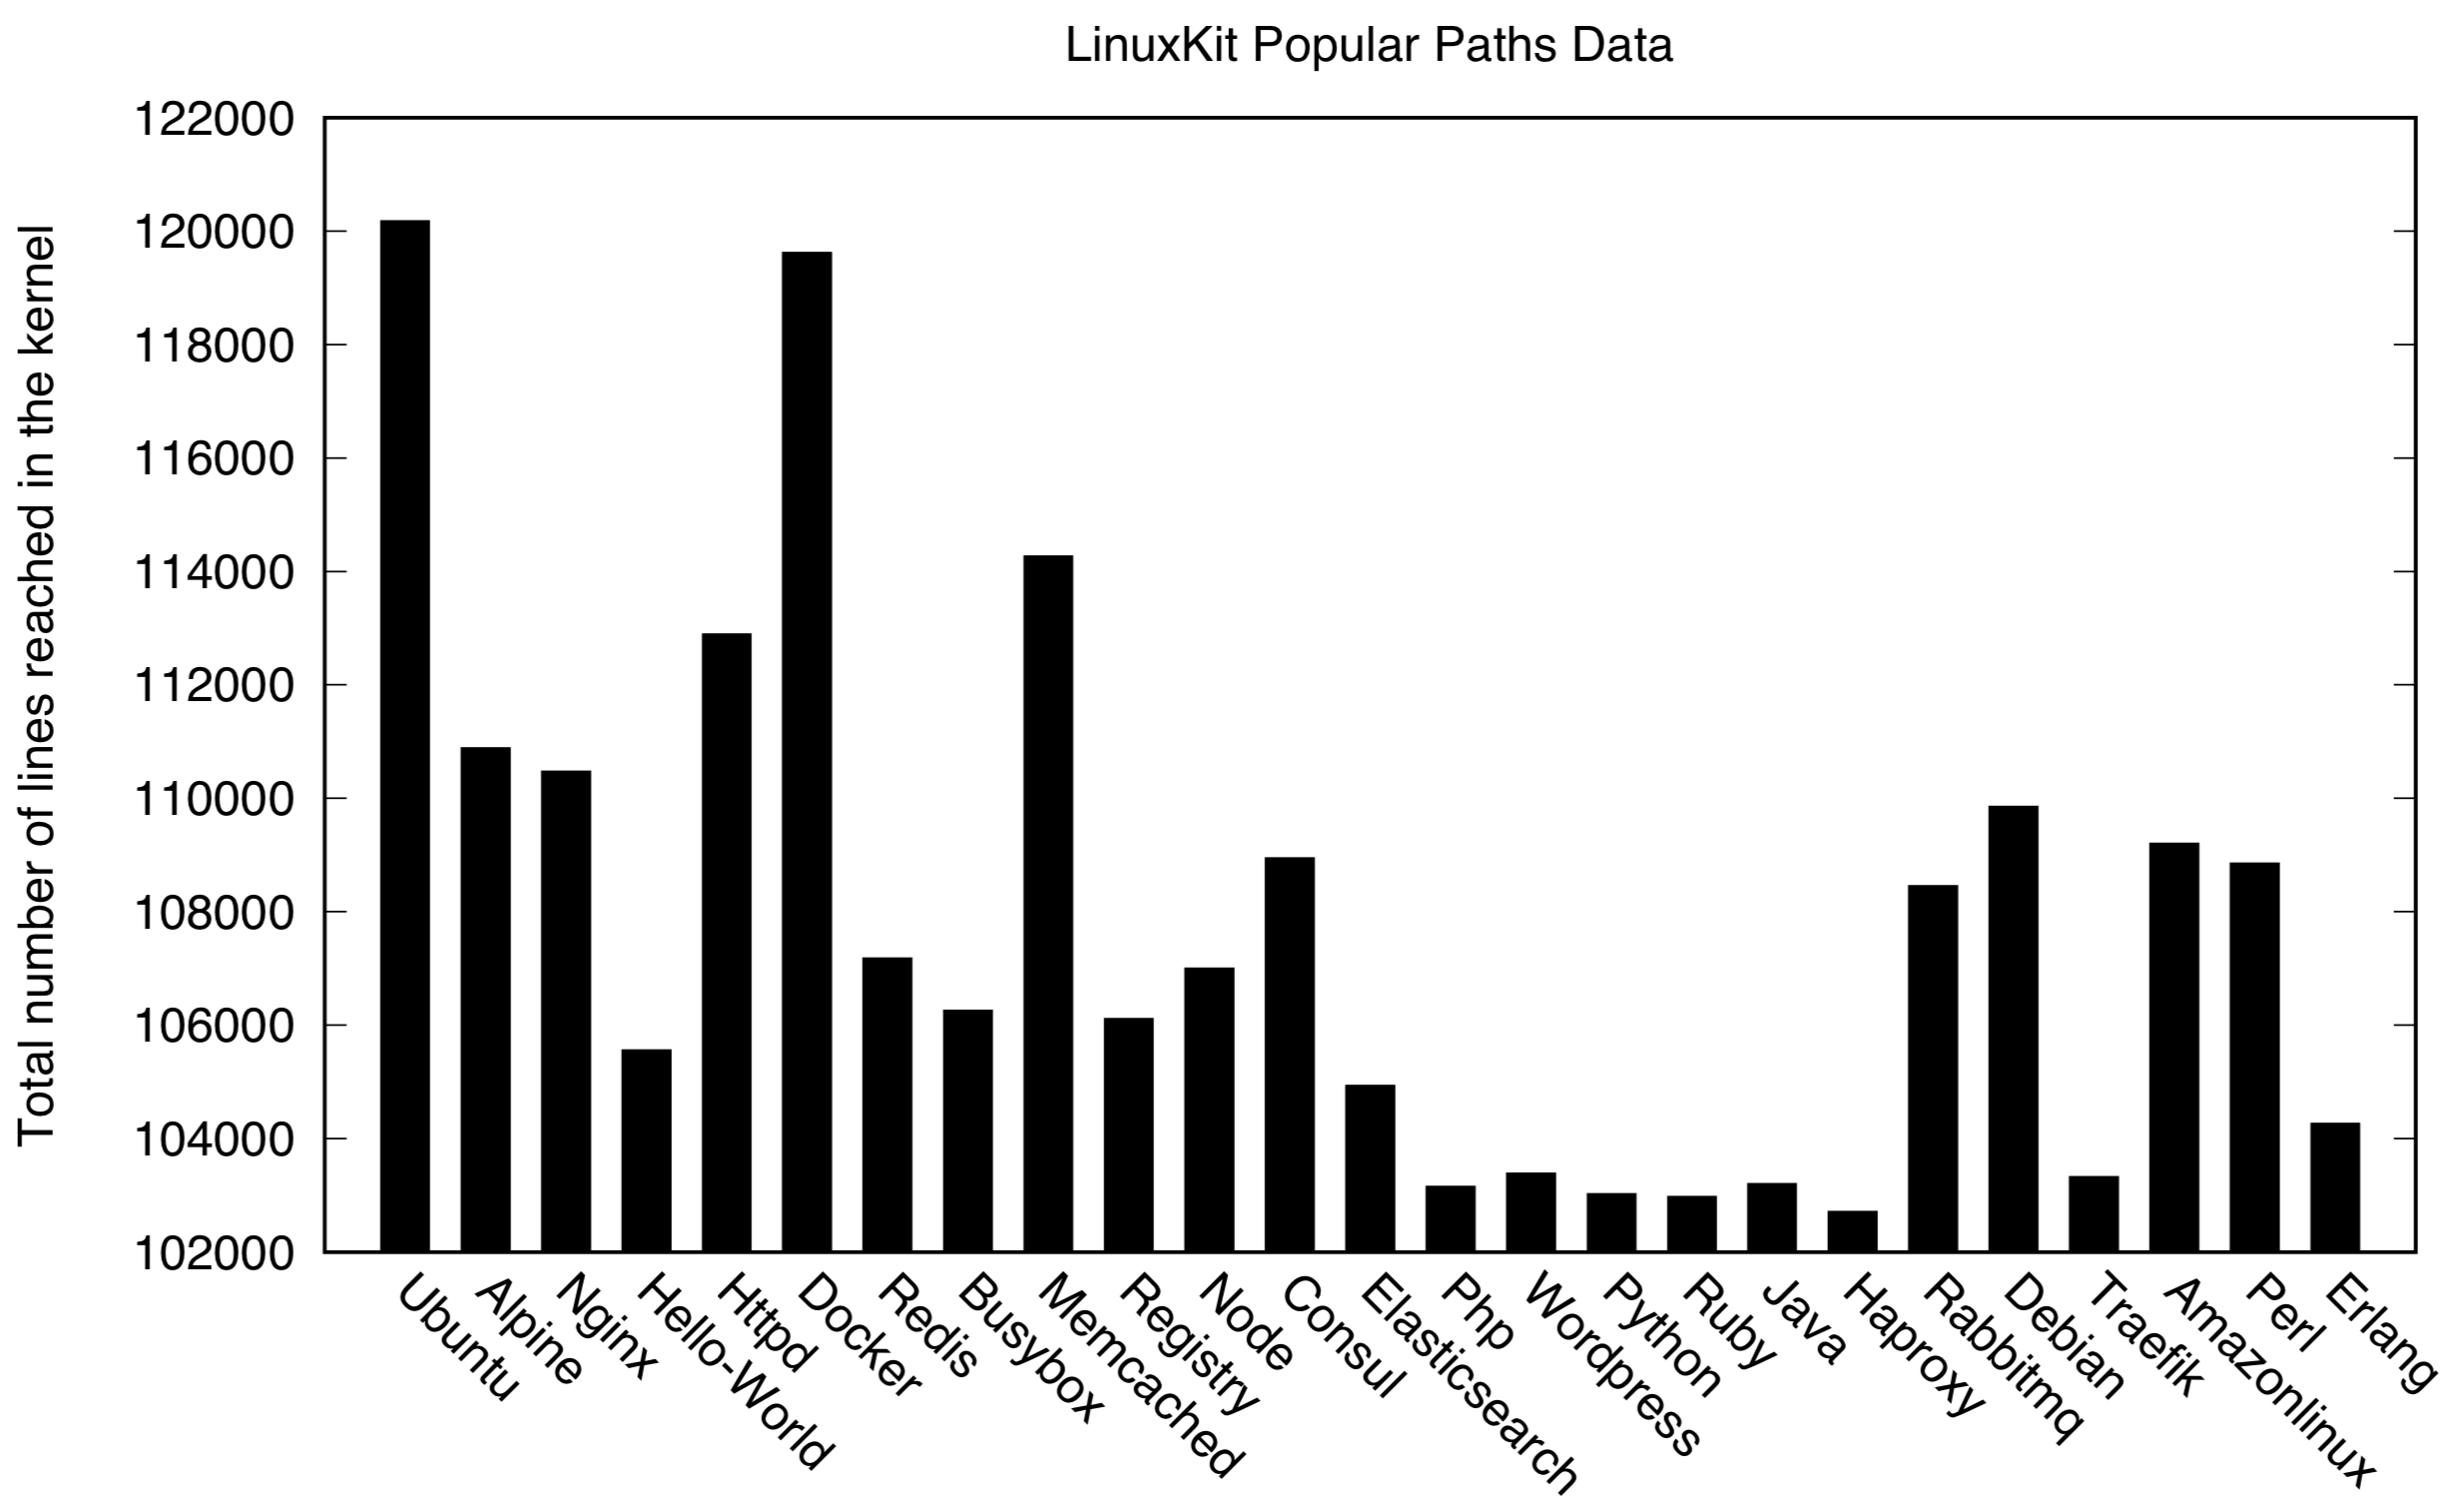
\includegraphics[width=1.5\columnwidth]{diagram/pp-individuals.png}
\caption{\small Popular paths for individual Docker containers}
\label{fig:pp-individuals}
\end{figure*}

\begin{figure*}
\centering
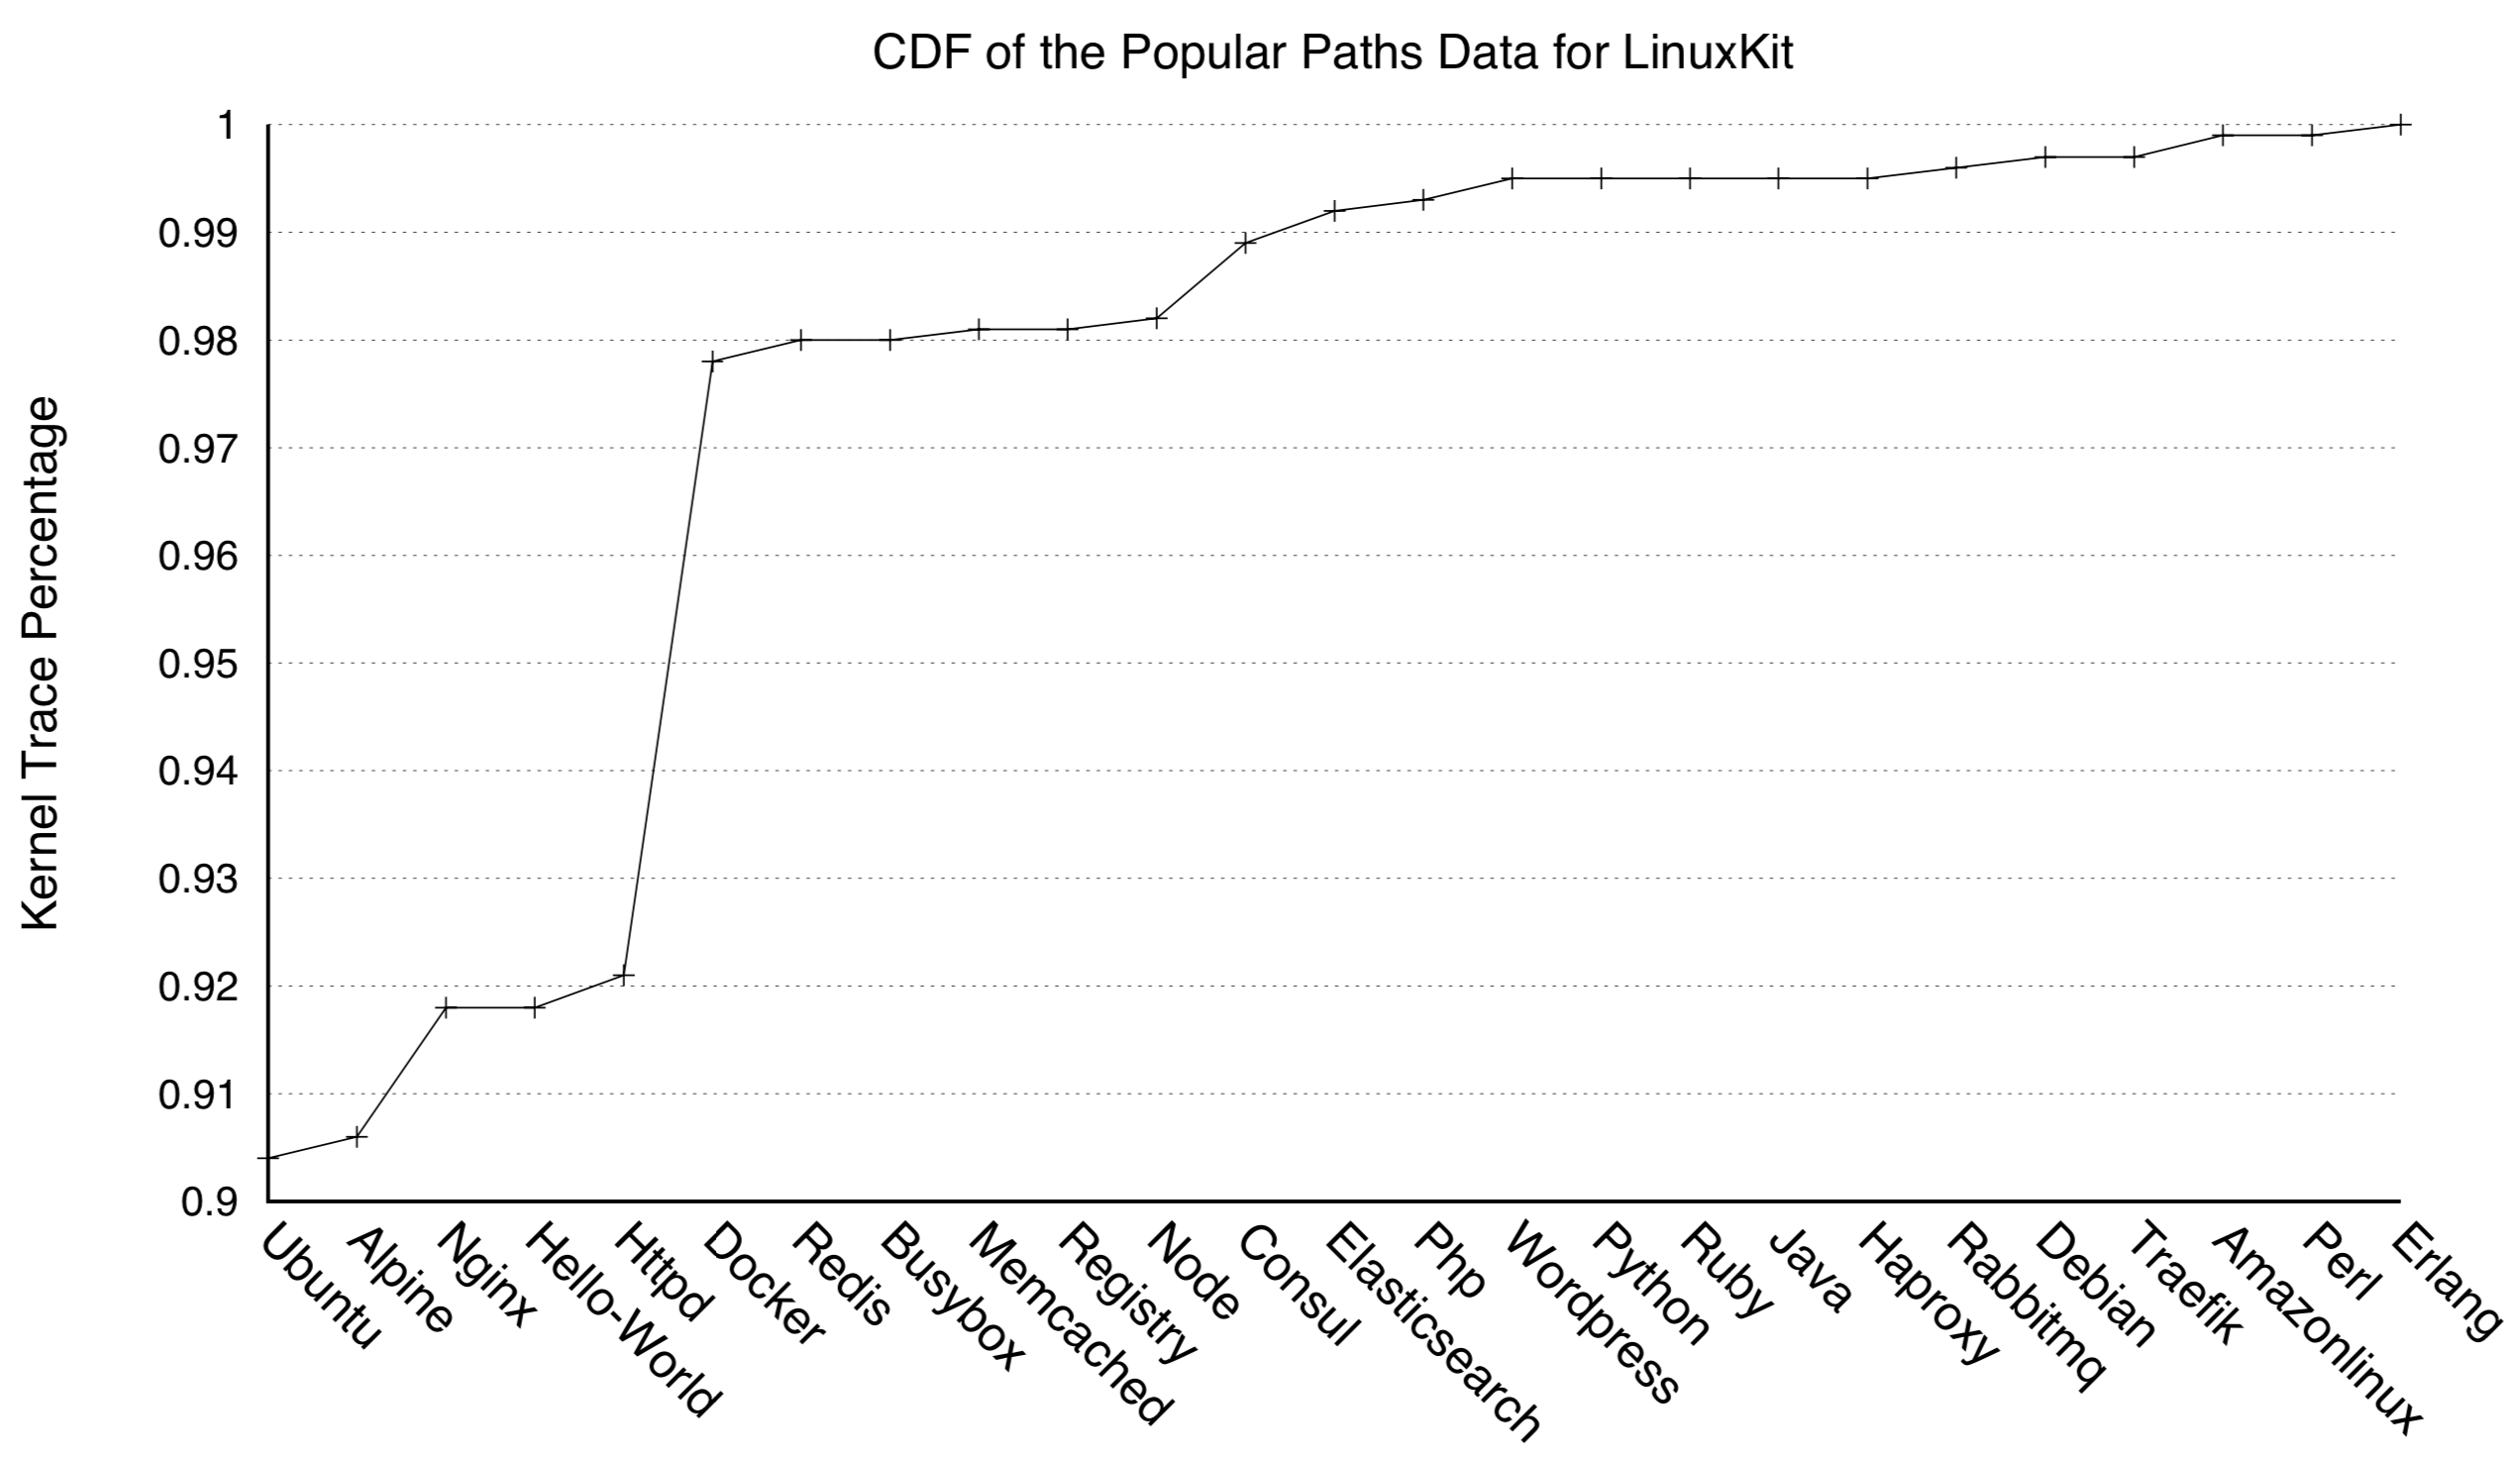
\includegraphics[width=1.5\columnwidth]{diagram/pp-cdf.png}
\caption{\small CDF of the popular paths of Docker containers showing most share the same kernel footprint}
\label{fig:pp-cdf}
\end{figure*}

\begin{figure*}
\centering
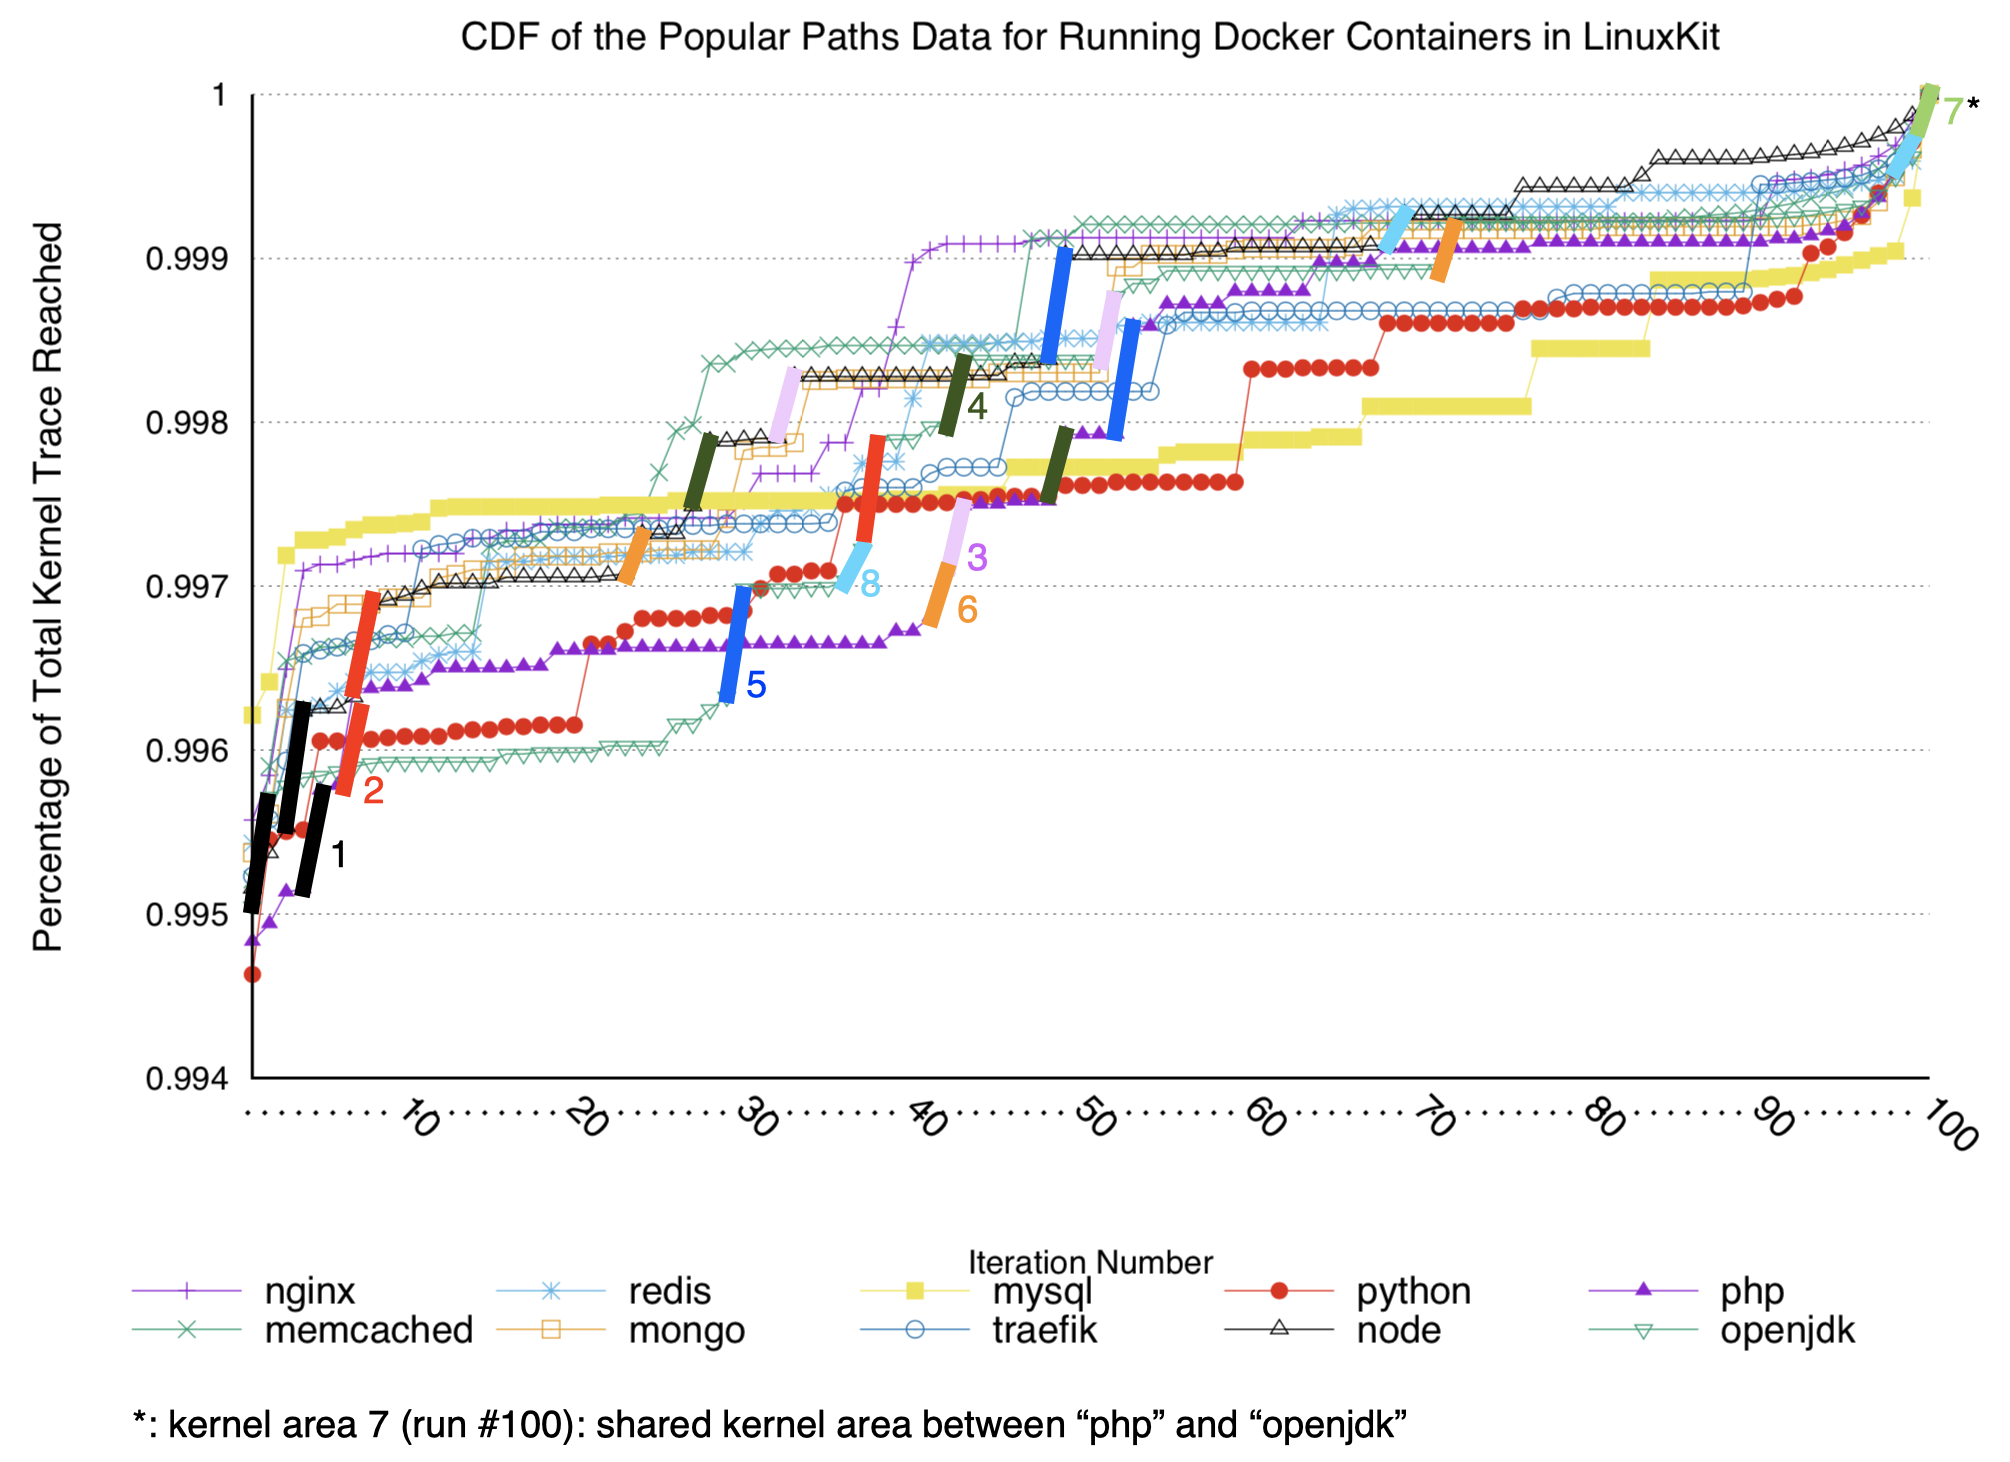
\includegraphics[width=1.5\columnwidth]{diagram/cdf-marked.png}
\caption{\small Common kernel code identified across different containers}
\label{fig:cdf-marked}
\end{figure*}

\subsubsection{Testing functionality on real-world container applications}
\label{sec.evaluation.functionality.containers} 
\textbf{Experimental Setup.}
To confirm that our Secure Logging Kernel works in real-world practices, we tested the 100 most downloaded containers from Docker Hub. 
We ran the experiment in the same version of the LinuxKit virtual machine as in 4.1.1. 
Each Docker container was run in the LinuxKit VM using the commands in its Dockerfile from its official Docker image. 
To take into account any potential variances, each container was run in the exact same environment for 10 times. 

\textbf{Results.}
One of the more important results of this initial test was that it showed most containers shared the same kernel footprint. 
This means that the kernel trace, or the record of all kernel code executed, of a sample of containers can represent the trace of many more. 
We used the CDF (Cumulative Distribution Function) to analyze how soon the kernel trace of different containers would converge. 
Results of the CDF, as visualized  in Figure \ref{fig:pp-cdf}, 
points out that the trace of the top six popular containers covered about 98\% of the total kernel trace for 25 containers. 
This offers additional corroboration that the popular paths data we collected is valid not only for the few containers we ran, but also for hundreds of containers on Docker Hub.  

In addition to the always used popular paths, which we identified as the common kernel lines that appeared each and every time, 
we also discovered certain lines of kernel code that showed up sporadically. 
For these lines, we looked at what activities they performed, and how common they were across different containers. 
In our analysis of the kernel trace of 10 popular Docker containers, we identified eight pieces of infrequently executed kernel code common among them. 
These traces are presented graphically in Figure \ref{fig:cdf-marked}. 
Each numbered line (from 1 to 8) in the graph represents a piece of infrequently executed code. 
The kernel function that corresponds with each of the eight pieces is explained below: 
\begin{enumerate}
	\item \verb|kernel/cgroup/freezer.c|: a cgroup is freezing if any FREEZING flags are set.
	\item \verb|kernel/locking/rwsem-xadd.c|: waiting for a write lock to be granted. 
	\item \verb|kernel/locking/rwsem-xadd.c|: waiting for the read lock to be granted.
	\item \verb|mm/filemap.c|: process waitqueue for pages and check for a page match to prevent potential waitqueue hash collision. 
	\item \verb|fs/exec.c|: all other threads have exited, wait for the thread group leader to become inactive and to assume its PID. 
	\item \verb|kernel/workqueue|: insert a barrier work in the queue. According to the comments from the kernel source code, 
	the reason for inserting a barrier work seems to be to prevent a cancellation. 
	This is because \\
	\verb|try_to_grab_pending()| can not determine whether the work to be grabbed is at the head of the queue and thus can not clear LINKED flag of the previous work. 
	There must be a valid next work after a work with a LINKED flag set. 
	\item \verb|arch/x86/kernel/tsc.c|: try to calibrate the TSC \\ 
	against the Programmable Interrupt Timer and return the frequency of the TSC in kHz. 
	\item \verb|kernel/locking/mutex.c|: hand off a mutex. Give up ownership to a specific task, when @task = NULL, this is equivalent to a regular unlock.
\end{enumerate}

What this analysis tells us is that this infrequently used code performs essential kernel functions used by multiple containers, and therefore should still be considered popular paths, 
despite the fact that they are infrequently execute. 
On closer examination, we learn they are not always executed during each run because they are race-condition related code that depend on locks, and system conditions may vary during different runs. 
As the Secure Logging System profiles and identifies these infrequently-executed popular paths, as well as the always-executed ones, 
our tests show that the Secure Logging Kernel functions in a correct manner.

\begin{table*}[h!]
\begin{center}
\caption{Instrumentation code added in our Secure Logging Kernel}
\label{tab:kernel_instrumentation}
\begin{tabular}{c|c|c|c}
 kernel dir & unpopular functions & popular functions & total lines inserted \\
 \hline
 arch & 1502 & 931 & 3325 \\
 \hline
 block & 774 & 245 & 1035 \\
 \hline
 crypto & 527 & 121 & 656 \\ 
 \hline
 drivers & 6290 & 2584 & 13305 \\
 \hline
 fs & 2108 & 1404 & 4883 \\
 \hline
 ipc & 198 & 42 & 249 \\
 \hline
 kernel & 3721 & 2120 & 6335 \\
 \hline
 mm & 1037 & 792 & 2954 \\
 \hline
 net & 4107 & 1746 & 7510 \\
 \hline
 security & 200 & 180 & 551 \\
 \hline
 \textbf{total} & \textbf{20464} & \textbf{10165} & \textbf{40803} \\
\end{tabular}
\end{center}
\end{table*}

Based on the comprehensive popular paths data obtained, the Secure Logging System was able to create a customized Secure Logging Kernel for the LinuxKit VM. 
Table \ref{tab:kernel_instrumentation} presents an overview of the required modifications. 

Using  the Secure Logging Kernel, we ran the 100 containers and verified that they were able to finish their normal workloads, 
as defined in their official Dockerfiles, with, on average, less than 1\% of runtime overhead. 
In doing so, the containers used less than 0.1\% of the unpopular paths. 
A total number of 50 lines of unpopular paths were reached and recorded by the Secure Logging Kernel. 
This data strongly argues the feasibility of creating a popular-paths based host kernel to run Docker containers. 
In other words, real-world containers can run on only the popular paths in most (>99.9\%) cases. 

\begin{table*}[h!]
  \begin{center}
    \caption{Evaluation of the CVE vulnerabilities for the Linux kernel}
    \label{tab:evaluation_cve}
    \begin{tabular}{c|l|c|c|c} % <-- Alignments: 1st column left, 2nd middle and 3rd right, with vertical lines in between
      \textbf{\#} & \textbf{CVE ID} & \textbf{CVSS Score} & \textbf{Description} & \textbf{Detected in the}\\
       & & & & \textbf{LinuxKit Popular Paths}\\
      \hline
      1 & CVE-2019-10124 & 7.8 & denial of service, in mm/memory-failure.c & \ding{55}\\
      2 & CVE-2019-9213 & 4.9 & kernel NULL pointer dereferences, in mm/mmap.c & \ding{55}\\
      3 & CVE-2019-9003 & 7.8 & use-after-free & \ding{55}\\
      4 & CVE-2019-8956 & 7.2 & use-after-free & \ding{55}\\
      5 & CVE-2019-8912 & 7.2 & use-after-free & \ding{55}\\
      6 & CVE-2019-7308 & 7.5 & out-of-bounds speculation on pointer arithmetic & \ding{55}\\
      7 & CVE-2019-3701 & 7.1& privilege escalation & \ding{55}\\
      8 & CVE-2018-1000204 & 6.3 & copy kernel heap pages to the userspace & \ding{55}\\
      9 & CVE-2018-1000200 & 4.9 & NULL pointer dereference & \ding{55}\\
      10 & CVE-2018-1000026 & 6.8 & denial of service & \ding{55}\\
      11 & CVE-2018-20511 & 2.1 & privilege escalation & \ding{55}\\
      12 & CVE-2018-20169 & 7.2 & mishandle size checks & \ding{55}\\
      13 & CVE-2018-18690 & 4.9 & unchecked error condition & \ding{55}\\
      14 & CVE-2018-18445 & 7.2 & out-of-bounds memory access & \ding{55}\\
      15 & CVE-2018-18281 & 4.6 & improperly flush TLB before releasing pages & \ding{55}\\
      16 & CVE-2018-18021 & 3.6 & denial of service & \ding{55}\\
      17 & CVE-2018-16862 & 2.1 & the cleancache subsystem incorrectly clears an inode & \ding{55}\\
      18 & CVE-2018-16658 & 3.6 & local attackers could read kernel memory & \ding{55}\\
      19 & CVE-2018-16276 & 7.2 & privilege escalation & \ding{55}\\
      \color{red}{20} & \color{red}{CVE-2018-15594} & \color{red}{2.1} & \color{red}{spectre-v2 attacks against paravirtual guests} & \color{red}{\ding{51}}\\
      \color{red}{21} & \color{red}{CVE-2018-15572} & \color{red}{2.1} & \color{red}{userspace-userspace spectreRSB attacks} & \color{red}{\ding{51}}\\
      22 & CVE-2018-14646 & 4.9 & NULL pointer dereference & \ding{55}\\
      23 & CVE-2018-14634 & 7.2 & integer overflow, privilege escalation & \ding{55}\\
      24 & CVE-2018-14633 & 8.3 & stack buffer overflow & \ding{55}\\
      25 & CVE-2018-14619 & 7.2 & privilege escalation & \ding{55}\\
      26 & CVE-2018-13406 & 7.2 & integer overflow & \ding{55}\\
      27 & CVE-2018-12904 & 4.4 & privilege escalation & \ding{55}\\
      28 & CVE-2018-11508 & 2.1 & local user could access kernel memory & \ding{55}\\
      29 & CVE-2018-11412 & 4.3 & ext4 incorrectly allows external inodes for inline data & \ding{55}\\
      30 & CVE-2018-10940 & 4.9 & incorrect bounds check allows kernel memory access & \ding{55}\\
      31 & CVE-2018-10881 & 4.9 & denial of service & \ding{55}\\
      32 & CVE-2018-10880 & 7.1 & denial of service & \ding{55}\\
      33 & CVE-2018-10879 & 6.1 & use-after-free & \ding{55}\\
      34 & CVE-2018-10878 & 6.1 & denial of service & \ding{55}\\
      35 & CVE-2018-10074 & 4.9 & denial of service & \ding{55}\\
      36 & CVE-2018-10021 & 4.9 & denial of service & \ding{55}\\
      37 & CVE-2018-8781 & 7.2 & code execution in kernel space & \ding{55}\\
      38 & CVE-2018-6555 & 7.2 & denial of service & \ding{55}\\
      39 & CVE-2018-6554 & 4.9 & denial of service & \ding{55}\\
      40 & CVE-2018-5390 & 7.8 & denial of service & \ding{55}\\
      41 & CVE-2018-1130 & 4.9 & NULL pointer dereference & \ding{55}\\
      \color{red}{42} & \color{red}{CVE-2018-1120} & \color{red}{3.5} & \color{red}{denial of service} & \color{red}{\ding{51}}\\
      43 & CVE-2018-1118 & 2.1 & kernel memory leakage & \ding{55}\\
      44 & CVE-2018-1068 & 7.2 & write to kernel memory & \ding{55}\\
      45 & CVE-2017-1000410 & 5.0 & leaking data in kernel address space & \ding{55}\\
      46 & CVE-2017-1000407 & 6.1 & denial of service & \ding{55}\\
      47 & CVE-2017-1000405 & 6.9 & overwrite read-only huge pages & \ding{55}\\
      48 & CVE-2017-18224 & 1.9 & race condition, denial of service & \ding{55}\\
      49 & CVE-2017-18216 & 2.1 & NULL pointer dereference, denial of service & \ding{55}\\
      50 & CVE-2015-5327 & 4.0 & out-of-bounds memory read & \ding{55}\\
    \end{tabular}
  \end{center}
\end{table*}

\begin{figure*}
\centering
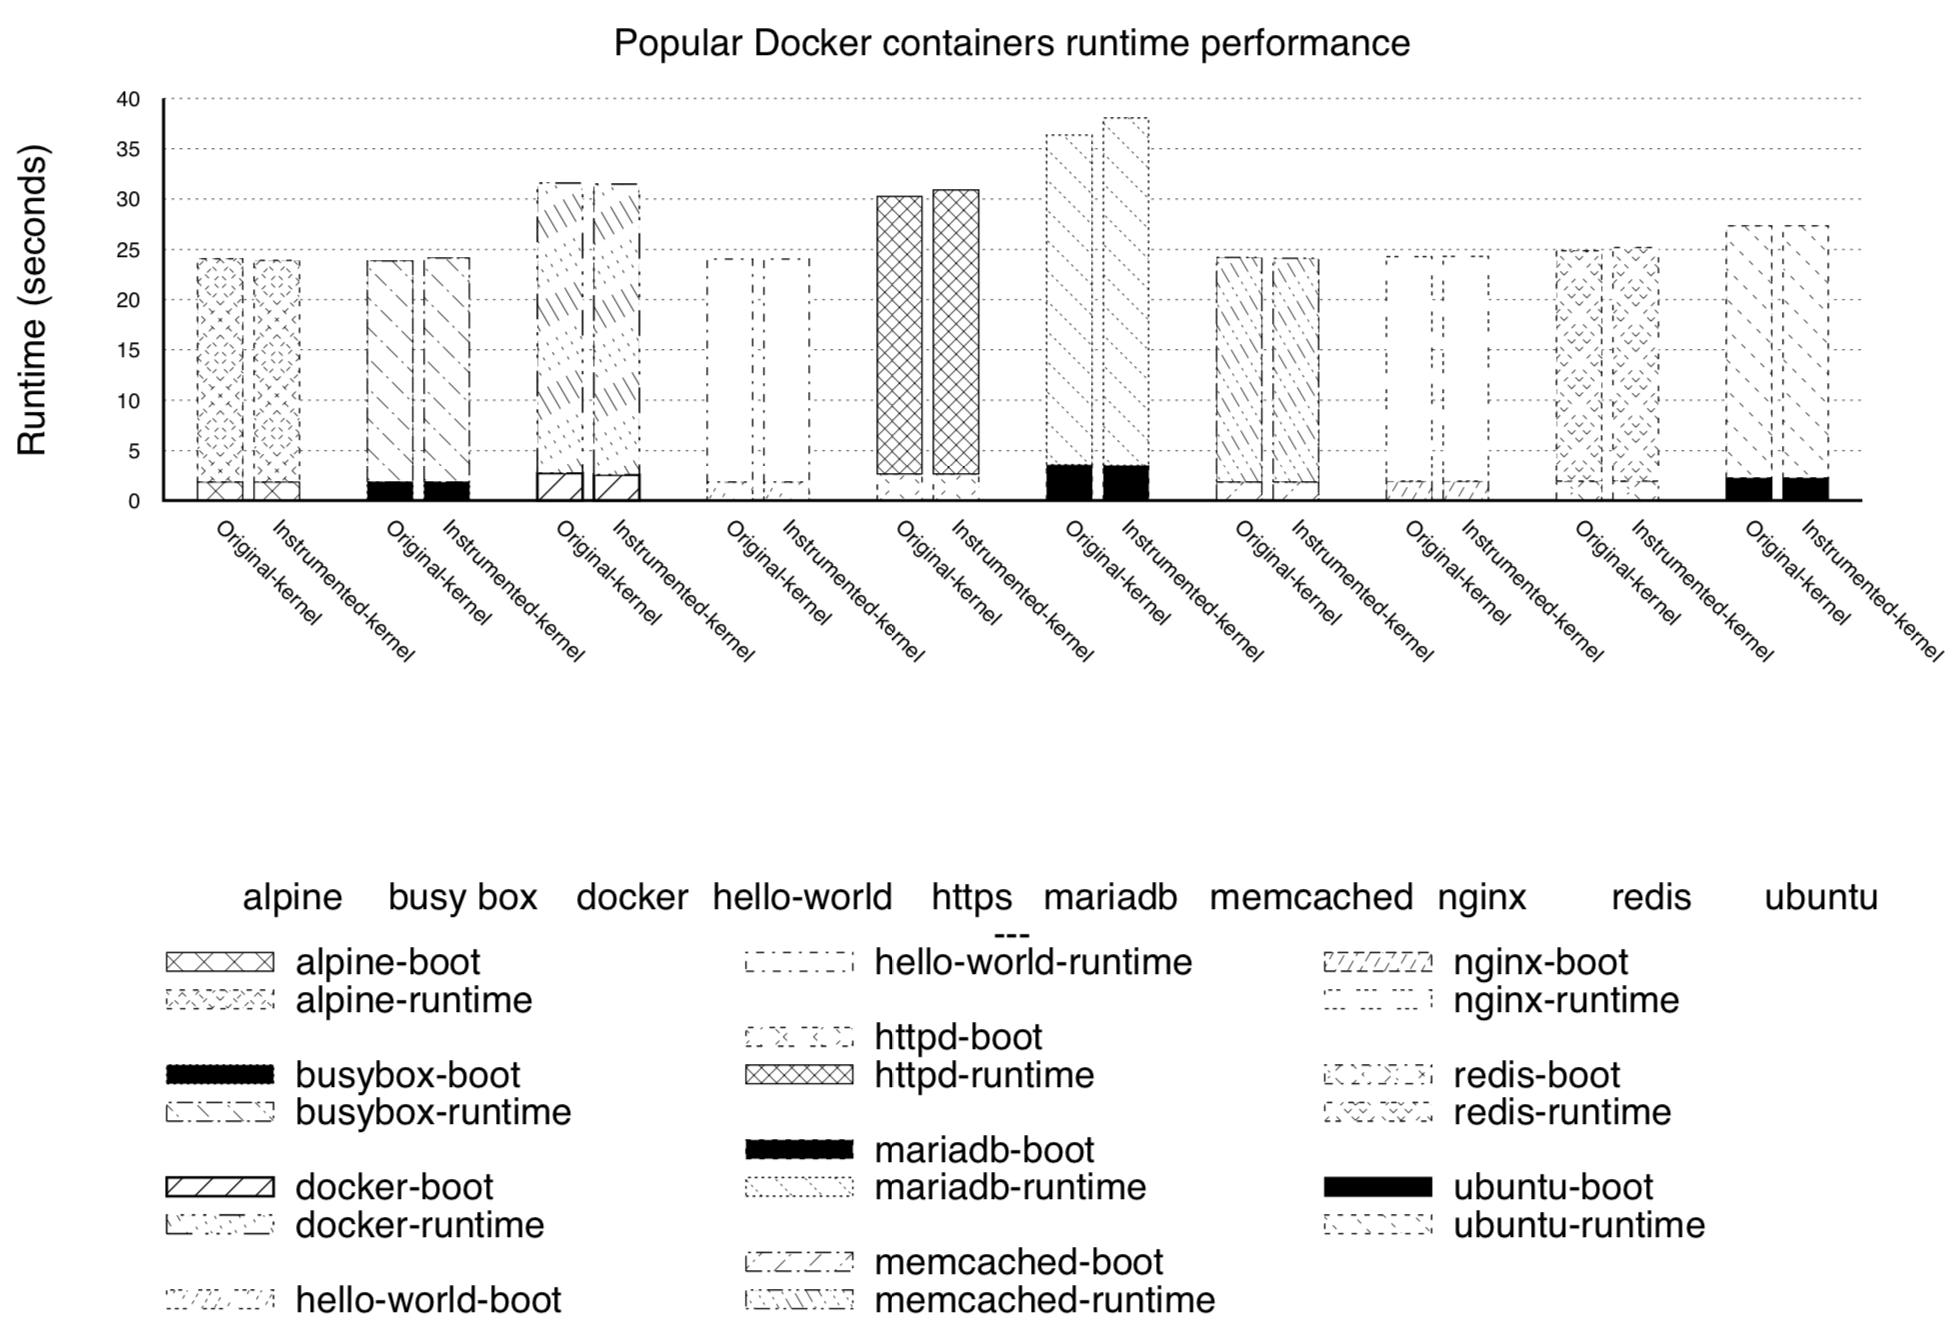
\includegraphics[width=1.5\columnwidth]{diagram/performance.png}
\caption{\small Runtime performance comparison for the top popular 10 containers}
\label{fig:performance}
\end{figure*}

\subsection{Security Evaluation}
\label{sec.evaluation.security} 
The main advantage of running containers on the popular paths is to leverage the security benefits. 
The popular paths have previously been proven to contain fewer security vulnerabilities. 
We want to verify if this still applies to containers in the face of new zero-day kernel vulnerabilities. 
The methodology we selected for this evaluation was to examine how many CVE kernel security bugs resided in the LinuxKit popular paths. 
If, as the metric suggests, there were fewer bugs in these paths, then our popular paths based solution would by its very design improve the security of running containers.

\textbf{Experimental Setup.}
We obtained a list of all the available (at the time of our study) CVE kernel vulnerabilities for Linux kernel version 4.14.x from the National Vulnerability Database. 
For each of these 50 vulnerabilities, we looked at the kernel patch that fixed the bug to identify the source line numbers that correspond to it. 
We then compared the line numbers against the popular paths kernel trace we had for LinuxKit to verify if the bug was present.

\textbf{Results.}
Out of the 50 CVE kernel security bugs we searched for, we found only three in the LinuxKit popular paths (lines occurred in any of the training runs), 
as shown in Table \ref{tab:evaluation_cve}. 
These three bugs were in commonly used kernel code that,   to the best of our knowledge, cannot be avoided by any existing security systems. 
We describe these three bugs in detail below to explain why they cannot be avoided, 
and to demonstrate that our popular paths based strategy did its best to reduce the risk of triggering kernel bugs.

\textbf{[CVE-2018-15594]}
This bug lies in \\
\verb|arch/x86/kernel/paravirt.c| in the Linux kernel before 4.18.1. 
The source code mishandles certain indirect calls, which makes it easier for attackers to conduct Spectre-v2 attacks against paravirtual guests. 
In our tests, this bug was found in the kernel trace data, and was reached frequently by programs running in LinuxKit, 
because the code inside of the \verb|paravirt_patch_call()| function in \\
\verb|arch/x86/kernel/paravirt.c| is used to rewrite an indirect call with a direct call, 
which is an essential function used to support the Linux kernel paravirtualization. 

\textbf{[CVE-2018-15572]}
The \verb|spectre_v2_select_mitigation| function in \verb|arch/x86/kernel/cpu/bugs.c| in the Linux kernel before 4.18.1 does not always fill RSB upon a context switch. 
This makes it easier for attackers to conduct userspace-userspace spectreRSB attacks. 
This piece of code in \\
\verb|spectre_v2_select_mitigation(void)| function would be used by every program, as the kernel attempts to mitigate potential Spectre attacks. 
Therefore any program that tries to mitigate the original Spectre attack would use this piece of code that contains this new CVE vulnerability. 
That's the reason why it appeared in our LinuxKit popular paths. 

\textbf{[CVE-2018-1120]}
This vulnerability was found affecting the Linux kernel before version 4.17. by \verb|mmap()|ing a FUSE-backed file onto 
the memory of a process containing command line arguments (or environment strings). 
This bug appeared in the popular paths because \verb|mmap()| is commonly used by user programs. 
Furthermore, this vulnerability involves \verb|proc_pid_cmdline_read()| and \verb|environ_read()| functions, that are commonly invoked by virtual machines and user programs.

By limiting the potential risk of exposure to kernel code to just these three bugs, the popular path metric already greatly reduces risks to container security. 
While a potential user of the popular paths metric must be aware of these bugs, 
the odds on having to deal with repeated and costly incidents from zero-day vulnerabilities become much more manageable.  

It should also be noted that 49 out of the 50 bugs tested were discovered and confirmed after publication of the original popular paths study \cite{Lock-in-Pop}, 
which shows that the metric can indeed predict where bugs are likely to occur effectively. 

\subsection{Performance Evaluation}
\label{sec.evaluation.performance} 
Lastly, we wanted to assure container users that utilizing our Secure Logging Kernel  would not negatively affect performance overhead costs. 
To demonstrate this, we evaluated both the run-time performance and memory space overhead of the modified kernel.

\textbf{Experimental Setup.}
In order to measure the overhead costs of our Secure Logging Kernel, 
we did a comparison between containers running on the original Linux kernel and ones running on our popular-paths based kernel. 
We used the exact same running environment and configuration to ensure a fair comparison. 
We ran the 100 most popular containers from Docker Hub on both the original kernel and our Secure Logging Kernel. 
In each test, the container finished its workload as defined in the official Dockerfile. We measured the runtimes for both kernels and compared them. 

\textbf{Results.}
Our results show that, on average, running containers on our popular-paths based kernel incurred about 0.5\% to 1\% of extra performance overhead as compared to the original Linux kernel. Results of the top 10 containers are shown in Figure \ref{fig:performance}.

The original Linux kernel image used for the  LinuxKit test  is sized at 163,012,008 bytes . 
In comparison, the popular-paths based kernel is sized at 163,622,440 bytes. Therefore, the extra memory space added by our modified kernel was only about 0.37\%. 

Based on our performance evaluation, the Secure Logging Kernel has negligible overhead in both runtime and memory space. 